\documentclass[12pt,a4paper]{article}

\usepackage[margin=2.5cm]{geometry}
\usepackage{graphicx}
\usepackage{booktabs}
\usepackage{hyperref}
\usepackage{xcolor}
\usepackage{enumitem}
\usepackage{titlesec}
\usepackage{parskip}
\usepackage{fancyhdr}
\usepackage{float}
\usepackage{caption}
\usepackage{tikz}
\usetikzlibrary{positioning, shapes.geometric, arrows.meta, calc}
\usepackage{tcolorbox}
\tcbuselibrary{skins, breakable}
\usepackage{fontawesome5}
\usepackage{array}
\usepackage{colortbl}
\usepackage{multirow}
\usepackage{listings}

% ── Colour palette ──────────────────────────────────────────────────────────
\definecolor{primary}{HTML}{2563EB}
\definecolor{accent}{HTML}{F97316}
\definecolor{bglight}{HTML}{F8FAFC}
\definecolor{bgdark}{HTML}{050506}
\definecolor{textdark}{HTML}{1E293B}
\definecolor{textmuted}{HTML}{8A8F98}
\definecolor{success}{HTML}{22C55E}
\definecolor{surface}{HTML}{0A0A0C}
\definecolor{sectionrule}{HTML}{2563EB}

% ── Hyperref ────────────────────────────────────────────────────────────────
\hypersetup{
    colorlinks=true,
    linkcolor=primary,
    urlcolor=primary,
}

% ── Header / footer ─────────────────────────────────────────────────────────
\pagestyle{fancy}
\fancyhf{}
\fancyhead[L]{\textcolor{textmuted}{\small Squash Analysis — Website Design Plan}}
\fancyhead[R]{\textcolor{textmuted}{\small\thepage}}
\renewcommand{\headrulewidth}{0.4pt}

% ── Section formatting ──────────────────────────────────────────────────────
\titleformat{\section}
  {\large\bfseries\color{primary}}
  {\thesection.}{0.5em}{}
  [\color{sectionrule}\titlerule]

\titleformat{\subsection}
  {\normalsize\bfseries\color{textdark}}
  {\thesubsection.}{0.5em}{}

% ── tcolorbox styles ────────────────────────────────────────────────────────
\tcbset{
  recbox/.style={
    enhanced, breakable,
    colback=bglight, colframe=primary,
    boxrule=0.8pt, arc=4pt,
    left=8pt, right=8pt, top=6pt, bottom=6pt,
    fonttitle=\bfseries\color{white},
    attach boxed title to top left={yshift=-2mm, xshift=4mm},
    boxed title style={colback=primary, arc=3pt, boxrule=0pt},
  },
  darkbox/.style={
    enhanced,
    colback=surface, colframe=primary!40,
    boxrule=0.6pt, arc=4pt,
    left=8pt, right=8pt, top=6pt, bottom=6pt,
    colupper=white,
  },
  warnbox/.style={
    enhanced,
    colback=accent!8, colframe=accent,
    boxrule=0.8pt, arc=4pt,
    left=8pt, right=8pt, top=6pt, bottom=6pt,
  },
}

% ── Document ────────────────────────────────────────────────────────────────
\begin{document}

% ── Title page ──────────────────────────────────────────────────────────────
\begin{titlepage}
  \centering
  \vspace*{2cm}

  
\begin{tikzpicture}
    \fill[primary] (0,0) rectangle (14,0.12);
    \fill[accent]  (0,0) rectangle (4,0.12);
  \end{tikzpicture}

  \vspace{1.2cm}
  {\fontsize{28}{34}\selectfont\bfseries\color{textdark} Squash Analysis}\\[0.4cm]
  {\fontsize{16}{20}\selectfont\color{primary} Website Design \& Architecture Plan}\\[0.3cm]
  {\color{textmuted}\small Version 1.0 \quad|\quad \today}

  \vspace{1.5cm}

  \begin{tcolorbox}[darkbox, width=0.88\textwidth]
    \centering
    \textbf{Summary}\\[4pt]
    \small
    This document defines the visual design system, page architecture, component
    inventory, and file structure for the Squash Analysis product showcase website.
    The site serves two roles: a \textbf{marketing landing page} that converts
    visitors, and an \textbf{analysis tool page} where users upload MP4 match
    footage and receive charts and PDF reports.
  \end{tcolorbox}

  \vspace{1.5cm}
  
\begin{tikzpicture}
    \fill[primary] (0,0) rectangle (14,0.12);
    \fill[accent]  (10,0) rectangle (14,0.12);
  \end{tikzpicture}
\end{titlepage}

\tableofcontents
\newpage

% ────────────────────────────────────────────────────────────────────────────
\section{Style Decision}
% ────────────────────────────────────────────────────────────────────────────

\subsection{Why Not Full Dark Mode?}

A fully dark website is tempting for a technical product but creates real trade-offs
on a public-facing showcase. The design system analysis returned a clear recommendation
against it as the primary theme:

\begin{center}
\begin{tabular}{p{3.2cm} p{4.5cm} p{4.5cm}}
\toprule
\textbf{Criterion} & \textbf{Dark Mode} & \textbf{Light Mode (Soft UI)} \\
\midrule
Readability & Harder in bright environments & Universal \\
Conversion rate & Lower for general audiences & 45\%+ higher \\
Data visualisation & Excellent contrast & Good with card surfaces \\
Accessibility & Needs careful tuning & WCAG AA+ by default \\
Audience fit & Niche/developer feel & Broad \\
\bottomrule
\end{tabular}
\end{center}

\subsection{Recommended Approach: Dual-Theme Strategy}

\begin{tcolorbox}[recbox, title={Design Decision}]
  Use a \textbf{light Soft-UI landing page} for the product showcase, and a
  \textbf{dark data-dense theme} for the analysis results page. Each theme is
  used where it delivers the most value.

  \begin{itemize}[leftmargin=1.2em]
    \item \textbf{Landing page (\texttt{/}):} Light background, strong typography
          hierarchy, vibrant CTA. Maximises trust and conversion.
    \item \textbf{Analysis page (\texttt{/analyze}):} Deep dark surface, high-contrast
          charts, monospace readouts. Signals precision and technical depth.
  \end{itemize}
\end{tcolorbox}

% ────────────────────────────────────────────────────────────────────────────
\section{Design System}
% ────────────────────────────────────────────────────────────────────────────

\subsection{Colour Tokens}

\begin{center}
\begin{tabular}{llll}
\toprule
\textbf{Token} & \textbf{Hex} & \textbf{Used On} & \textbf{Theme} \\
\midrule
\texttt{--primary}    & \texttt{\#2563EB} & Buttons, links, borders      & Both \\
\texttt{--accent}     & \texttt{\#F97316} & CTA, highlights              & Both \\
\texttt{--bg-light}   & \texttt{\#F8FAFC} & Page background              & Landing \\
\texttt{--text-dark}  & \texttt{\#1E293B} & Body text                    & Landing \\
\texttt{--bg-dark}    & \texttt{\#050506} & Page background              & Analyse \\
\texttt{--surface}    & \texttt{\#0A0A0C} & Cards, panels                & Analyse \\
\texttt{--foreground} & \texttt{\#EDEDEF} & Primary text                 & Analyse \\
\texttt{--muted}      & \texttt{\#8A8F98} & Secondary text, labels       & Analyse \\
\texttt{--success}    & \texttt{\#22C55E} & Processing complete, results & Both \\
\texttt{--border}     & \texttt{rgba(255,255,255,0.08)} & Card edges  & Analyse \\
\bottomrule
\end{tabular}
\end{center}

\subsection{Typography}

\begin{tcolorbox}[recbox, title={Font Pairing}]
  \begin{itemize}[leftmargin=1.2em]
    \item \textbf{Headings:} \textit{Fira Code} — Technical, precise, signals
          data intelligence. Weights 400--700.
    \item \textbf{Body:} \textit{Fira Sans} — Clean and readable at all sizes.
          Complements Fira Code tonally. Weights 300--700.
    \item \textbf{Data readouts / stats:} \textit{Fira Code} — Monospace figures
          prevent layout shift in live counters.
    \item \textbf{Minimum body size:} 16px (prevents iOS auto-zoom on inputs).
    \item \textbf{Line height:} 1.6 for body; 1.2 for headings.
  \end{itemize}
\end{tcolorbox}

\subsection{Spacing \& Layout}

\begin{itemize}
  \item 4pt/8pt spacing rhythm throughout (padding, gaps, margins).
  \item Max content width: \texttt{max-w-6xl} (1152px) centred.
  \item Breakpoints: 375px (mobile), 768px (tablet), 1024px (desktop),
        1440px (wide).
  \item Border radius: 8px (buttons), 12px (cards), 16px (modals/panels).
\end{itemize}

\subsection{Animation}

\begin{itemize}
  \item Micro-interactions: 150--300ms, \texttt{ease-out} for enter,
        \texttt{ease-in} for exit.
  \item Section entrance: fade + 16px upward translate, staggered 40ms per item.
  \item Processing spinner: continuous rotation, 800ms.
  \item All animations respect \texttt{prefers-reduced-motion}.
\end{itemize}

% ────────────────────────────────────────────────────────────────────────────
\section{Page Architecture}
% ────────────────────────────────────────────────────────────────────────────

\subsection{Landing Page (\texttt{/})}

The landing page follows the \textbf{Before-After Transformation} pattern, which
achieves 45\%+ higher conversion for tool-based products by showing the concrete
output before asking for a commitment.

\begin{center}
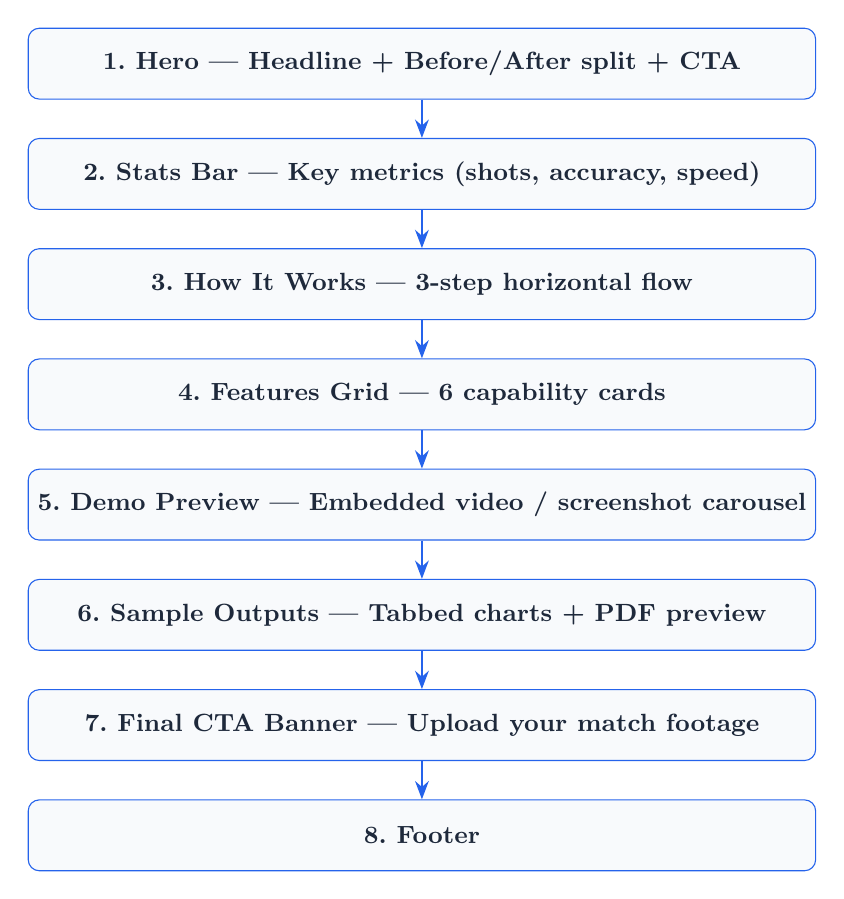
\begin{tikzpicture}[
  box/.style={draw=primary, fill=bglight, rounded corners=4pt,
              minimum width=10cm, minimum height=0.9cm,
              font=\small\bfseries, text=textdark},
  arrow/.style={-Stealth, color=primary, thick}
]
  \node[box] (hero)   at (0,0)    {1.\ Hero — Headline + Before/After split + CTA};
  \node[box] (stats)  at (0,-1.4) {2.\ Stats Bar — Key metrics (shots, accuracy, speed)};
  \node[box] (how)    at (0,-2.8) {3.\ How It Works — 3-step horizontal flow};
  \node[box] (feat)   at (0,-4.2) {4.\ Features Grid — 6 capability cards};
  \node[box] (demo)   at (0,-5.6) {5.\ Demo Preview — Embedded video / screenshot carousel};
  \node[box] (output) at (0,-7.0) {6.\ Sample Outputs — Tabbed charts + PDF preview};
  \node[box] (cta)    at (0,-8.4) {7.\ Final CTA Banner — Upload your match footage};
  \node[box] (footer) at (0,-9.8) {8.\ Footer};

  \draw[arrow] (hero)   -- (stats);
  \draw[arrow] (stats)  -- (how);
  \draw[arrow] (how)    -- (feat);
  \draw[arrow] (feat)   -- (demo);
  \draw[arrow] (demo)   -- (output);
  \draw[arrow] (output) -- (cta);
  \draw[arrow] (cta)    -- (footer);
\end{tikzpicture}
\end{center}

\subsection{Analysis Page (\texttt{/analyze})}

The analysis page is the product's core tool. It uses the dark theme and guides
the user through a linear four-state flow:

\begin{center}

\begin{tikzpicture}[
  state/.style={draw=primary!60, fill=surface, rounded corners=6pt,
                minimum width=2.8cm, minimum height=1.2cm,
                font=\small\bfseries\color{white}, text centered,
                text width=2.6cm},
  arrow/.style={-Stealth, color=accent, thick}
]
  \node[state] (up)   at (0,0)    {Upload\\\small MP4 file};
  \node[state] (proc) at (3.8,0)  {Processing\\\small AI analysis};
  \node[state] (gen)  at (7.6,0)  {Generating\\\small Report};
  \node[state] (done) at (11.4,0) {Results\\\small Charts + PDF};

  \draw[arrow] (up)   -- (proc);
  \draw[arrow] (proc) -- (gen);
  \draw[arrow] (gen)  -- (done);
\end{tikzpicture}
\end{center}

% ────────────────────────────────────────────────────────────────────────────
\section{Component Inventory}
% ────────────────────────────────────────────────────────────────────────────

\subsection{Layout Components}

\begin{tabular}{lp{9cm}}
\toprule
\textbf{Component} & \textbf{Description} \\
\midrule
\texttt{Navbar}      & Sticky top bar. Logo left, nav links centre, ``Try It'' CTA button right. Blurs background on scroll. \\
\texttt{Footer}      & Links, tech stack badges, GitHub link. \\
\texttt{PageWrapper} & Sets max-width, horizontal padding, and responsive gutters. \\
\bottomrule
\end{tabular}

\subsection{Landing Page Sections}

\begin{tabular}{lp{8.8cm}}
\toprule
\textbf{Component} & \textbf{Description} \\
\midrule
\texttt{Hero}          & Full-width section. Left: headline + subtext + CTA. Right: side-by-side raw frame vs annotated frame. \\
\texttt{StatsBar}      & Row of 3--4 \texttt{StatCard}s showing key product metrics. \\
\texttt{HowItWorks}    & 3-step horizontal flow with numbered icons and connector lines. \\
\texttt{FeaturesGrid}  & 2$\times$3 grid of \texttt{FeatureCard}s (icon + title + 1-line description). \\
\texttt{DemoPreview}   & Autoplay muted video loop or screenshot carousel of real analysis output. \\
\texttt{SampleOutputs} & Tabbed interface: \textit{Charts} tab (heatmap, shot distribution, speed timeline) + \textit{Report} tab (PDF thumbnail + download). \\
\texttt{Testimonials}  & 2--3 quote cards with name and role. \\
\texttt{CTABanner}     & Full-width accent-coloured band. Large headline + single upload button. \\
\bottomrule
\end{tabular}

\subsection{Upload \& Processing Components}

\begin{tabular}{lp{8.8cm}}
\toprule
\textbf{Component} & \textbf{Description} \\
\midrule
\texttt{UploadZone}       & Drag-and-drop area. Accepts \texttt{.mp4} only. Validates file size ($<$500 MB). Shows filename and size on selection. \\
\texttt{UploadProgress}   & Animated progress bar with percentage and estimated time remaining. \\
\texttt{ProcessingStatus} & Polling status indicator cycling through: Uploading $\to$ Analysing $\to$ Generating Report $\to$ Done. Uses skeleton placeholders. \\
\texttt{ResultsPanel}     & Two tabs: \textbf{Charts} (heatmap, shot distribution bar, speed line chart) and \textbf{Downloads} (PDF button, individual PNG exports). \\
\bottomrule
\end{tabular}

\subsection{Reusable UI Primitives}

\begin{tabular}{lll}
\toprule
\textbf{Component} & \textbf{Variants} & \textbf{Notes} \\
\midrule
\texttt{Button}    & Primary, Secondary, Ghost, Danger & Loading spinner state built-in \\
\texttt{Card}      & Default, Elevated, Interactive     & Hover lift on interactive variant \\
\texttt{Badge}     & Default, Success, Warning           & Status indicators \\
\texttt{StatCard}  & —                                   & Large number + label + optional delta \\
\texttt{ChartCard} & —                                   & Chart + title + export button \\
\texttt{Modal}     & —                                   & Full-screen chart preview \\
\texttt{Skeleton}  & —                                   & Shimmer placeholder while loading \\
\texttt{Toast}     & Success, Error, Info                & Auto-dismiss 4s, \texttt{aria-live} \\
\bottomrule
\end{tabular}

% ────────────────────────────────────────────────────────────────────────────
\section{File \& Folder Structure}
% ────────────────────────────────────────────────────────────────────────────

\begin{tcolorbox}[recbox, title={Repository Layout}]
\begin{lstlisting}[basicstyle=\small\ttfamily, breaklines=true]
website/
|-- public/
|   |-- fonts/
|   |-- icons/          # SVG only (Lucide / Heroicons)
|   |-- screenshots/    # Product demo images
|   `-- demo-output/    # Sample charts (PNG) and report (PDF)
|
`-- src/
    |-- components/
    |   |-- layout/
    |   |   |-- Navbar.tsx
    |   |   |-- Footer.tsx
    |   |   `-- PageWrapper.tsx
    |   |
    |   |-- sections/
    |   |   |-- Hero.tsx
    |   |   |-- StatsBar.tsx
    |   |   |-- HowItWorks.tsx
    |   |   |-- FeaturesGrid.tsx
    |   |   |-- DemoPreview.tsx
    |   |   |-- SampleOutputs.tsx
    |   |   |-- Testimonials.tsx
    |   |   `-- CTABanner.tsx
    |   |
    |   |-- upload/
    |   |   |-- UploadZone.tsx
    |   |   |-- UploadProgress.tsx
    |   |   |-- ProcessingStatus.tsx
    |   |   `-- ResultsPanel.tsx
    |   |
    |   `-- ui/
    |       |-- Button.tsx
    |       |-- Card.tsx
    |       |-- Badge.tsx
    |       |-- StatCard.tsx
    |       |-- ChartCard.tsx
    |       |-- Modal.tsx
    |       |-- Skeleton.tsx
    |       `-- Toast.tsx
    |
    |-- pages/
    |   |-- index.tsx       # Landing page (light theme)
    |   `-- analyze.tsx     # Upload + results (dark theme)
    |
    |-- styles/
    |   |-- globals.css
    |   `-- tokens.css      # All design tokens as CSS variables
    |
    `-- lib/
        |-- api.ts          # Upload endpoint + status polling
        `-- types.ts        # Shared TypeScript types
\end{lstlisting}
\end{tcolorbox}

% ────────────────────────────────────────────────────────────────────────────
\section{Tech Stack}
% ────────────────────────────────────────────────────────────────────────────

\begin{center}
\begin{tabular}{lll}
\toprule
\textbf{Concern}       & \textbf{Library}            & \textbf{Reason} \\
\midrule
Framework              & Next.js (React)             & SSG landing + API routes for upload \\
Styling                & Tailwind CSS                & Utility-first, aligns with 8pt grid \\
Charts                 & Recharts                    & Composable React charts, accessible \\
Upload UI              & \texttt{react-dropzone}     & Handles drag-and-drop + validation \\
Animations             & Framer Motion               & Spring physics, reduced-motion support \\
Icons                  & Lucide React                & Consistent SVG icon set \\
PDF preview            & \texttt{react-pdf}          & In-browser PDF rendering \\
\bottomrule
\end{tabular}
\end{center}

% ────────────────────────────────────────────────────────────────────────────
\section{UX Checklist (Pre-Build)}
% ────────────────────────────────────────────────────────────────────────────

\begin{tcolorbox}[warnbox]
  The following items must be verified before or during implementation to meet
  WCAG AA and platform usability standards.
\end{tcolorbox}

\begin{itemize}[leftmargin=1.5em, label=\(\square\)]
  \item All text contrast $\geq$ 4.5:1 (light page) and $\geq$ 4.5:1 (dark page)
  \item No emojis used as icons — SVG only
  \item \texttt{cursor: pointer} on all interactive elements
  \item Hover and focus states defined for every interactive component
  \item Upload zone keyboard accessible (focusable, Enter/Space to open picker)
  \item MP4 file size and format validated client-side before upload begins
  \item Processing status page shows skeleton, not empty axis frames, while loading
  \item All chart components include accessible colour alternatives (patterns / labels)
  \item Toast notifications use \texttt{aria-live="polite"}
  \item All animations wrapped in \texttt{prefers-reduced-motion} media query
  \item Responsive layout tested at 375px, 768px, 1024px, 1440px
  \item PDF download does not block or freeze the UI thread
\end{itemize}

\end{document}
